\documentclass[]{scrartcl}

\usepackage{float}
\usepackage{pgfplots}
\usepackage{xparse}
\usepackage{mathtools}
\usepackage{amsmath}
\usepackage{graphicx} % Required for including pictures
\usepackage{wrapfig} % Allows in-line images
\usepackage{url}
\usepackage{mathpazo} % Use the Palatino font
\usepackage[T1]{fontenc} % Required for accented characters
\linespread{1.05} % Change line spacing here, Palatino benefits from a slight increase by default

\DeclarePairedDelimiter\ceil{\lceil}{\rceil}
\DeclarePairedDelimiter\floor{\lfloor}{\rfloor}
\makeatletter
\newcommand{\mathleft}{\@fleqntrue\@mathmargin0pt}
\newcommand{\mathcenter}{\@fleqnfalse}
\renewcommand\@biblabel[1]{\textbf{#1.}} % Change the square brackets for each bibliography item from '[1]' to '1.'
\renewcommand{\@listI}{\itemsep=0pt} % Reduce the space between items in the itemize and enumerate environments and the bibliography

\renewcommand{\maketitle}{ % Customize the title - do not edit title and author name here, see the TITLE block below
	\begin{center} % Right align
		{\LARGE\@title} % Increase the font size of the title
		
		\vspace{15pt} % Some vertical space between the title and author name
		{\large\@author} % Author name
		\\\@date % Date
		
	\end{center}
}

\usepackage{xcolor}
\usepackage{textcomp}
\definecolor{dkgreen}{rgb}{0,0.6,0}
\definecolor{gray}{rgb}{0.5,0.5,0.5}
\definecolor{mauve}{rgb}{0.58,0,0.82}

\usepackage{listings}

%opening
\title{SPHINCS Interim Report}
\author{Daniel Kirkpatrick\\Vedanth Narayanan}

\begin{document}

\maketitle


\section*{Introduction}
Over the past 7 weeks, we have been focusing on SPHINCS for our project. Most of the work leading up to the past couple weeks have been reading documents that explain the tools being used in SPHINCS. The single biggest challenge for us was primarily getting acquainted with the material. To properly, and throughly, understand SPHINCS we needed to get caught up with a lot of reading. There were multiple papers that required time and dedication to fully understand. Understanding the tools and technologies is crucial if we want to be successful. On top of this, we had the added challenge of figuring out how to piece together the technologies, and how SPHINCS uses them.\\
While we had a lot of catching up to do, we also did get a chance to work on something new. The actual focus is transcribed in this paper. With help from Professor Yavuz, our goal was to come up with a simpler signature scheme that withheld the security that can be incorporated into SPHINCS. The scheme we propose is called Lamport+.

\section*{Preliminaries}
\vspace{-0.3cm}This section is utilized to briefly talk about existing signature schemes. The sole reason for this is so future references to the specific schemes are not ambiguous. 

\subsection*{Lamport Signature Scheme}
The Lamport Signature Scheme was created by Leslie Lamport in 1989, and it is the simplest signature scheme that exists. It is also the first One-Time signature that was invented. This scheme makes use of a cryptographic hash function that has already been predetermined.\\
To put it simply, the idea behind the scheme can be split into two separate pieces. Signer first generates the secret keys, public keys, hashes messages, and gets a signature that is passed off to the verifier. Now, the verifier's job more or less is to follow similar steps so they end up with a similar result. Thus, it can be argued that the message and signature could only come from the signer and no one else. The detailed version of the scheme is mentioned in the Lamport+ section.

\subsection*{WOTS}
The primary idea behind the scheme is to break the messages into little blocks, that get processed together, and having an input run through a hash function several times. The number of iterations entirely depends on the message that needs to be signed.\\
WOTS was built on top of the Lamport signature scheme, and the expectation is for it to be intuitive in its logic, but it's not the case. The complexity of the scheme is heavily influences by figuring out the number of iterations necessary for a value to go through the hash function.

\subsection*{WOTS+}
WOTS+ is very similar to WOTS, expect for the addition of XORing random elements every time a value is iterated over hash function. In the key generation phase, WOTS+ generates a set of random numbers that will serve for XORing. Just like the keys are split into chunks, so are the random elements. They get incorporated in the following recursive chaining function
\begin{equation}
c_{k}^{i}(x,\textbf{r}) = f_{k}(c_{k}^{i-1}(x,\textbf{r}) \oplus r_{i})
\end{equation}
Th equation is strictly $i > 0$, but in the case of $i = 0$, $c_{0}^{k}(x,\textbf{r}) = x$. The equation is clever in that it makes sure to XOR different values for every iteration. 

\section*{Lamport+ Signature Scheme}
Lamport+ Signature Scheme is the new scheme we are proposing. It not only brings the simplicity of the original Lamport scheme, but also pulls in elements of the WOTS+ scheme. Our hope is that the original scheme's security is withheld, if not enhanced. Please note that the security of the proposed scheme has not been proven, but it can very well be inferred from the previous. Similar to how WOTS+ introduces XORing of randomized elements to WOTS, the same principle is introduced to Lamport. The following is meant to give an idea of the new scheme before we extrapolate it to hash chains.\\ \\
\textbf{\textit{Key Pair Generation}}: $n$ is the number of random pairs to be generated. Random element $r \in \{0,1\}^n$ is chosen. The secret key is $sk = ((sk_{0,0}, sk_{0,1}),(sk_{1,0}, sk_{1,1}),...,(sk_{n,0}, sk_{n,1}))$. Each key is $n$-bits long. Let $f_k : \{0,1\}^n \rightarrow \{0,1\}^n | k \in \mathcal{K}_n$. The cryptographic hash function $f_k$ outputs a $n$-bit value. Public keys are derived by $pk = f_k(sk_{0,1} \oplus r)$. The whole set of $sk$ is run through the hash function, so get a bijective public key set. The public key is the following 
\mathleft
\begin{equation}
\begin{split}
pk & = ((pk_{0,0}, pk_{0,1}),(pk_{1,0}, pk_{1,1}),...,(pk_{n,0}, pk_{n,1})) \\
& = ((f_k(sk_{0,0} \oplus r), f_k(sk_{0,1}\oplus r)),(f_k(sk_{1,0} \oplus r), f_k(sk_{1,1}\oplus r)),...,\\
& \hspace{0.65cm}(f_k(sk_{n,0} \oplus r), f_k(sk_{n,1}\oplus r)))
\end{split}
\end{equation} \\
\textbf{\textit{Signature Generation}}: The message to be signed is $m$. This messaged is hashed by $h(m) = f_k(m \oplus r)$. For consistency purposes, we assume that the message size and $r$ are the same. The output of the hash is now $n$-bits. Based on every single bit (0 or 1), the corresponding key from a bit pair is selected from the secret keys. These keys make up the signature of the message.\\ \\
\textbf{\textit{Signature Verification}}: At this point, the verification is almost trivial. The verifier first obtains the hash of the message (once again, w). Based on the bits of the hash, they pick out the corresponding keys from public key of the signer. Now the signature that the signer gave the verifier is hashed, and ideally the values should equal the values that the verifier picked out of the public key. If and when the values don't match is when we know something is wrong. Also, make a note that when something is hashed, the random element is XORed in. Thus, the random element $r$ is passed off by the signer.

\subsection*{Lamport+ Hash Chain}
Hash chains aid One-Time signatures to be used multiple times with a single key. This can be applied to the Lamport+ signature scheme. The underlining idea here is that after the public key is generated in the scheme, another set of keys are generated based on the previous public key getting hashed. \\
There are two important things to make note of here. First off, we introduce a new parameter, which we call $l \in \mathbb{N}$, $l > 0$. This parameter helps keep track of how long the chain is, or many times new public keys have been derived. The second change involves generating a new randomized element for every new hashed public key. The random element from the previous level should not be used again. Now $\textbf{r}$ is a set, $\textbf{r} = (r_1,r_2,...,r_l)$. Once again, this concept is borrowed from WOTS+, where the random element changes based on the iteration number.\\
To properly use this hash chain, it's important to know the end of the chain. Imagine the length of the chain is 10. This chain can sign 10 messages. To verify a message, the 9th key down the chain is released. The $l$ parameter should then be decremented. When another message needs to be signed, then the 8th key should be released, and $l$ should be decremented. Once $l$ hits 0, there are no more messages that can be used. The random elements set does not need to be modified, because the subset $r_{1,...,l}$ automatically changes.

\subsection*{Lamport+ Hash Tree}
Note that this section hasn't been fully developed yet, and it is still in the works. If Lamport+ is going to get incorporated into SPHINCS, then it needs to be in a tree fashion. The idea we have is that the leafs of a Binary hash tree have the public keys of the hash chains. If there are four leaves, then there are 4 hash chain associated with each of the leaves. The parent node is a hash of the children hash nodes concatenated with each other, and XORed with a set of random elements for every level. The root node serves is the global public key.\\
When a signature is used from one of the leaves, then the tree needs to be computed again. Note that the whole tree does not need to be recomputed, but only the path to the specific leaf that used a signature. This idea hasn't been thought over entirely yet, but we believe that it should carry over.

\section*{Testing of SPHINCS, RSA, and ECDSA}
In this section we will be looking at the performance of SPHINCS, RSA, and ECDSA. These three cryptosystems each sign and verify messages in different ways. Below goes into a quick overview on how each system works. Below is a summary of each the cryptosystems we will be looking at. In the next section we will look at how these three cryptosystems match up against each other.

\subsection*{SPHINCS}
SPHINCS makes use of multiple trees to obtain a few time signature (FTS) scheme. This is done using a mixture of Winternitz one time signatures + (WOTS+) and HORS with trees (HORST). The idea of SPHINCS uses a hyper-tree which is borrowed from an idea by Goldreich, which turns a stateful scheme into a stateless scheme. WOTS+ eventually feeds into multiple HORST in the end, which allows for extending signatures to be multi-use instead of single use. SPHINCS has three steps: Key generation, signature generation and signature verification.

\subsection*{RSA}
RSA is used for signing messages by using public-key cryptography. It is an asymmetric cryptosystem that is based on the difficulty of factoring two large prime numbers. With RSA there are four steps we go through: key generation, key distribution, encryption and decryption.

\subsection*{ECDSA}
ECDSA uses elliptic-curve cryptography to obtain the needed parameters. Key generation in ECDSA requires less bits compared to DSA to obtain the same amount of security. The signature size requires the same amount of bit in both ECDSA and DSA to obtain the same amount of security. ECDSA contains three steps: Key generation, signature generation, and signature verification.

\section*{Benchmarks for SPHINCS, RSA, and ECDSA}
Benchmarking is done on Arch Linux (4.4.1-2-ARCH), processor: Intel Quad-Core i7-4710HQ 2.50GHz, 8 gigabytes RAM). The testing for SPHINCS is done using a python implementation that is not designed for optimization. This implementation was meant to learn and understand how individual pieces of SPHINCS work [1]. There are optimized versions of SPHINCS available, but compiling the from these implementations are very complex. The testing for RSA and ECDSA is done using MIRACL crypto library, which is an optimized library for performance [2].

The benchmarking is ran using different files sizes, ranging from 10 Kb up to 100 Kb with file sizes being increased in 10 Kb increments. Below you will find two different tests for each cryptosystem, signing and verification.

\begin{table} [H]
	\centering
	\caption{Performance of message signing}
	\begin{tabular}{|c|c|c|c|}
		\hline 
		& SPHINCS & RSA & ECDSA \\ 
		\hline 
		10 Kb & 1m 43.597sec & 0.005320ms & 0.000299ms \\ 
		\hline 
		20 Kb & 1m 42.665sec & 0.009426ms & 0.000480ms \\ 
		\hline 
		30 Kb & 1m 42.878sec & 0.013967ms & 0.000574ms \\ 
		\hline 
		40 Kb & 1m 43.089sec & 0.019238ms & 0.000687ms \\ 
		\hline 
		50 Kb & 1m 42.976sec & 0.023722ms & 0.000911ms \\ 
		\hline 
		60 Kb & 1m 43.105sec & 0.029159ms & 0.000921ms \\ 
		\hline 
		70 Kb & 1m 43.738sec & 0.032512ms & 0.001048ms \\ 
		\hline 
		80 Kb & 1m 44.051sec & 0.037693ms & 0.001293ms \\ 
		\hline 
		90 Kb & 1m 43.296sec & 0.042439ms & 0.002060ms \\ 
		\hline 
		100 Kb & 1m 43.495sec & 0.047571ms & 0.001676ms \\ 
		\hline 
	\end{tabular} 
\end{table}

\begin{table} [H]
	\centering
	\caption{Performance of message verification}
	\begin{tabular}{|c|c|c|c|}
		\hline 
		& SPHINCS & RSA & ECDSA \\ 
		\hline 
		10 Kb & 1.250sec & 0.000097ms & 0.001306ms \\ 
		\hline 
		20 Kb & 1.232sec & 0.000098ms & 0.001342ms \\ 
		\hline 
		30 Kb & 1.3sec & 0.000090ms & 0.001531ms \\ 
		\hline 
		40 Kb & 1.288sec & 0.000111ms & 0.001573ms \\ 
		\hline 
		50 Kb & 1.318sec & 0.000105ms & 0.001759ms \\ 
		\hline 
		60 Kb & 1.292sec & 0.000111ms & 0.001859ms \\ 
		\hline 
		70 Kb & 1.343sec & 0.000099ms & 0.002030ms \\ 
		\hline 
		80 Kb & 1.394sec & 0.000102ms & 0.002429ms \\ 
		\hline 
		90 Kb & 1.383sec & 0.000093ms & 0.002274ms \\ 
		\hline 
		100 Kb & 1.407sec & 0.000113ms & 0.002447ms \\ 
		\hline 
	\end{tabular} 
\end{table}

Below we will see the data put into another form which might be easier to comprehend the overall performance of each cryptosystem.

\begin{center}
	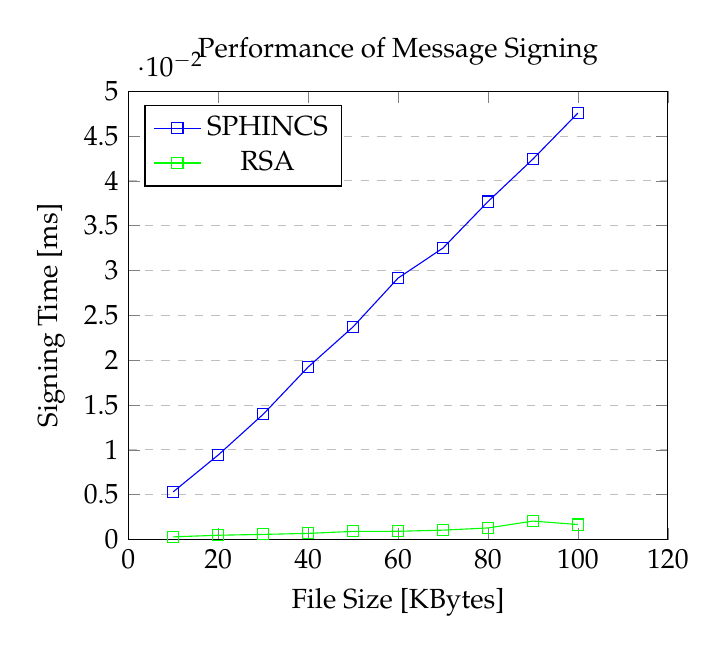
\begin{tikzpicture}
	\begin{axis}[
	title={Performance of Message Signing},
	xlabel={File Size [KBytes]},
	ylabel={Signing Time [ms]},
	xmin=0, xmax=120,
	ymin=0, ymax=0.050000,
	xtick={0,20,40,60,80,100,120},
	ytick={0, 0.005 ,0.010 ,0.015 ,0.020, 0.025, 0.030, 0.035, 0.040, 0.045, 0.050},
	legend pos=north west,
	ymajorgrids=true,
	grid style=dashed,
	]
	
	\addplot[
	color=blue,
	mark=square,
	]
	coordinates {(10,0.005320)(20,0.009426)(30,0.013967)(40,0.019238)(50,0.023722)(60,0.029159)(70,0.032512)(80,0.037693)(90,0.042439)(100,0.047571)
	};
	
	\addplot[
	color=green,
	mark=square,
	]
	coordinates {(10,0.000299)(20,0.000480)(30,0.000574)(40,0.000687)(50,0.000911)(60,0.000921)(70,0.001048)(80,0.001293)(90,0.002060)(100,0.001676)
	};
	
	\legend{SPHINCS, RSA, ECDSA}
	
	\end{axis}
	\end{tikzpicture}
\end{center}

\begin{center}
	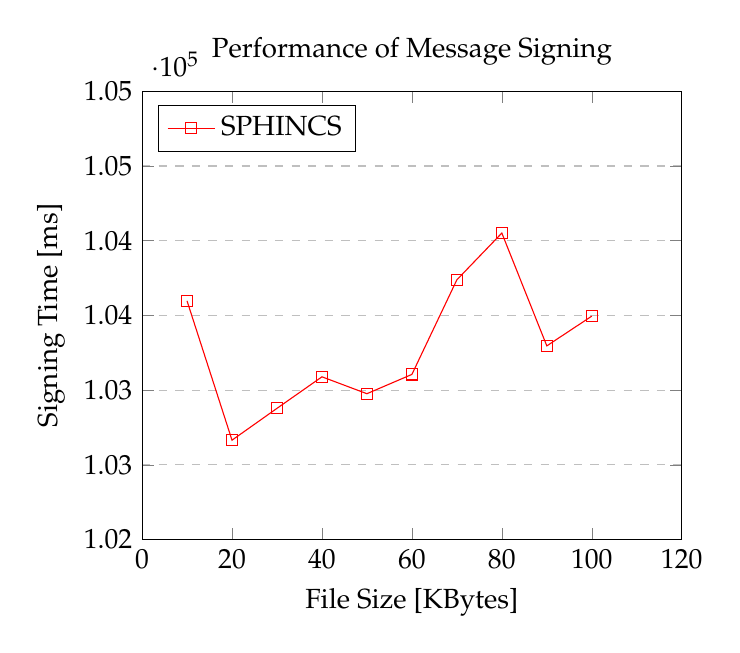
\begin{tikzpicture}
	\begin{axis}[
	title={Performance of Message Signing},
	xlabel={File Size [KBytes]},
	ylabel={Signing Time [ms]},
	xmin=0, xmax=120,
	ymin=102000, ymax=105000,
	xtick={0,20,40,60,80,100,120},
	ytick={0,102000,102500,103000,103500,104000,104500,105000},
	legend pos=north west,
	ymajorgrids=true,
	grid style=dashed,
	]
	
	\addplot[
	color=red,
	mark=square,
	]
	coordinates {(10,103597)(20,102665)(30,102878)(40,103089)(50,102976)(60,103105)(70,103738)(80,104051)(90,103296)(100,103495)
	};
	
	\legend{SPHINCS}
	
	\end{axis}
	\end{tikzpicture}
\end{center}

\begin{center}
	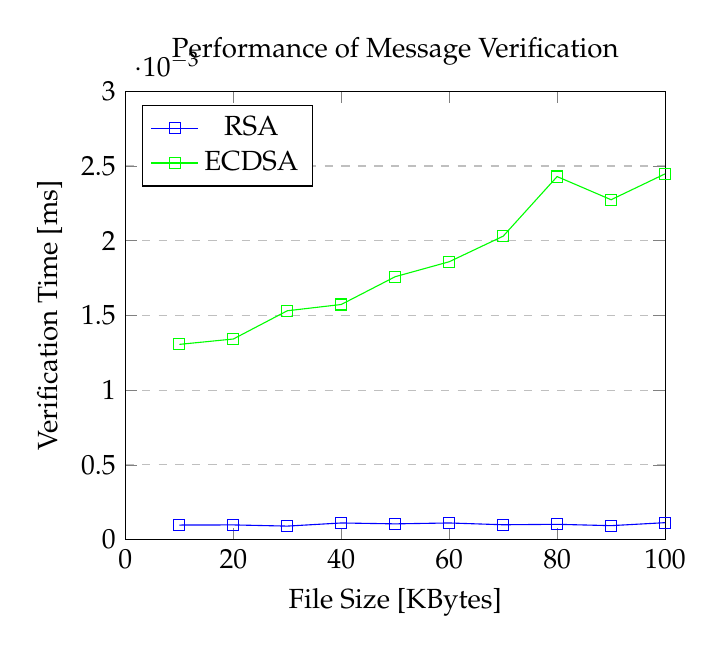
\begin{tikzpicture}
	\begin{axis}[
	title={Performance of Message Verification},
	xlabel={File Size [KBytes]},
	ylabel={Verification Time [ms]},
	xmin=0, xmax=100,
	ymin=0, ymax=0.003000,
	xtick={0,20,40,60,80,100},
	ytick={0, 0.0005 ,0.0010 ,0.0015 ,0.0020, 0.0025, 0.0030},
	legend pos=north west,
	ymajorgrids=true,
	grid style=dashed,
	]
	
	\addplot[
	color=blue,
	mark=square,
	]
	coordinates {(10,0.000097)(20,0.000098)(30,0.000090)(40,0.000111)(50,0.000105)(60,0.000111)(70,0.000099)(80,0.000102)(90,0.000093)(100,0.000113)
	};
	
	\addplot[
	color=green,
	mark=square,
	]
	coordinates {(10,0.001306)(20,0.001342)(30,0.001531)(40,0.001573)(50,0.001759)(60,0.001859)(70,0.002030)(80,0.002429)(90,0.002274)(100,0.002447)
	};
	
	\legend{RSA, ECDSA}
	
	\end{axis}
	\end{tikzpicture}
\end{center}

\begin{center}
	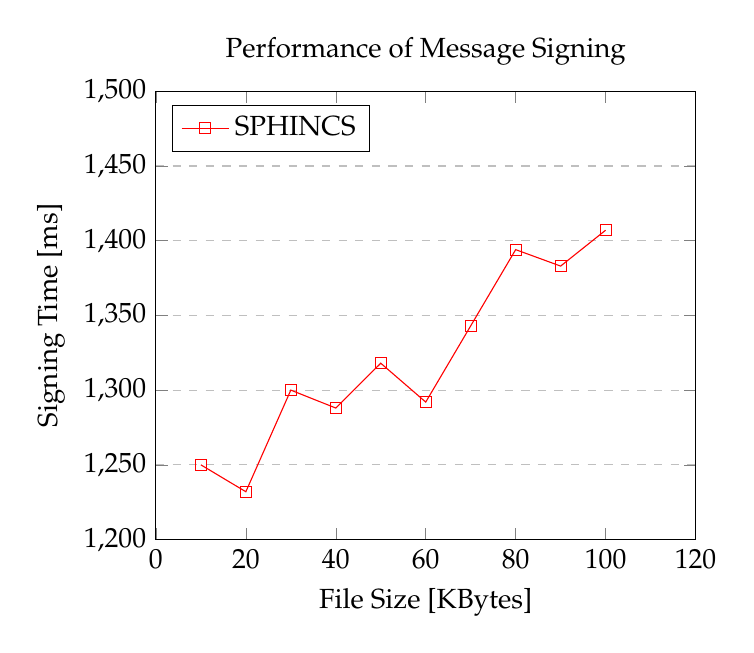
\begin{tikzpicture}
	\begin{axis}[
	title={Performance of Message Signing},
	xlabel={File Size [KBytes]},
	ylabel={Signing Time [ms]},
	xmin=0, xmax=120,
	ymin=1200, ymax=1500,
	xtick={0,20,40,60,80,100,120},
	ytick={0,1200,1250,1300,1350,1400,1450,1500},
	legend pos=north west,
	ymajorgrids=true,
	grid style=dashed,
	]
	
	\addplot[
	color=red,
	mark=square,
	]
	coordinates {(10,1250)(20,1232)(30,1300)(40,1288)(50,1318)(60,1292)(70,1343)(80,1394)(90,1383)(100,1407)
	};
	
	\legend{SPHINCS}
	
	\end{axis}
	\end{tikzpicture}
\end{center}

\textbf{NOTE:} Due to SPHINCS performance, it was placed into its own graphs. If it were included in the same graphs with RSA and ECDSA, then they would not be visible.

\section*{Conclusion}
In this report, we presented the Lamport+ Signature Scheme, which is much simpler than WOTS and WOTS+. WOTS+ is currently being used in SPHINCS. SPHINCS is indeed stateless, but if Lamport+ were to be integrated instead, the system would become stateful. We went through an example or two to make sure that the scheme worked and it was possible, but have not spent more time on it. We want to go over it again, and see how it fairs against edge cases and such. The plan is also to try to implement it, and integrate it with SPHINCS to see the results.\\
It must stressed, as stated in the Benchmarks section, the SPHINCS implementation that was used for this was not optimized at all. The reason for the use of this implementation of SPHINCS was due to ease of use. There are other optimized implementations available, but the complexity to use them is high.\\
With that being said, as you can see from the graphs above there are trade-offs with using any of these cryptosystems. As file sizes increase the time it takes to sign and verify messages will also increase.\\
Based on the implementations used for this benchmark, it would be best to use ECDSA for signatures. ECDSA performs faster than SPHINCS and RSA in terms of signing messages. As you can see though, RSA does verify messages faster than ECDSA, but if you look at the overall performance ECDSA is faster.

\section*{References}
\begin{enumerate}
\item Merkle, Ralph C. "A certified digital signature." Advances in Cryptology-CRYPTO'89 Proceedings. Springer New York, 1989.
\item Buchmann, Johannes, et al. "On the security of the Winternitz one-time signature scheme." Progress in Cryptology-AFRICACRYPT 2011. Springer Berlin Heidelberg, 2011. 363-378.
\item Hulsing, Andreas. "W-OTS+ Shorter signatures for hash-based signature schemes." Progress in Cryptology-AFRICACRYPT 2013. Springer Berlin Heidelberg, 2013. 173-188.
\item Bernstein, Daniel J., et al. "SPHINCS: practical stateless hash-based signatures." Advances in Cryptology-EUROCRYPT 2015. Springer Berlin Heidelberg, 2015. 368-397.
\item Buchmann, Johannes, et al. "CMSS - An improved Merkle signature scheme." Progress in Cryptology-INDOCRYPT 2006. Springer Berlin Heidelberg, 2006. 349-363.
\item Buchmann, Johannes, Erik Dahmen, and Andreas Hulsing. "XMSS-a practical forward secure signature scheme based on minimal security assumptions." Post-Quantum Cryptography. Springer Berlin Heidelberg, 2011. 117-129.
\item https://github.com/joostrijneveld/SPHINCS-py
\item https://github.com/CertiVox/MIRACL
\end{enumerate}

\end{document}
